\section{Resting atmosphere}
This two-dimensional test simulates a stably stratified atmosphere in hydrostatic balance.  Since there are no net forces, the analytical solution should remain at rest.  \TODO{again, what is this designed to test?  Klemp says the horiz pressure gradient}

\subsection{Specification}
Following \textcite{weller-shahrokhi2014}, the domain is \SI{20}{\kilo\meter} wide and \SI{20}{\kilo\meter} high, which is narrower than \textcite{klemp2011} in order to reduce simulation time.  The wave-shaped mountain profile is taken from \textcite{schaer2002} where the surface height $h$ is given by
\begin{align}
\surface(x) = \surface_0 \exp \left( - \left( \frac{x}{a} \right)^2 \right) \cos^2 \left( \frac{\pi x}{\lambda} \right)
\end{align}
where $a = \SI{5}{\kilo\meter}$ is the mountain half-width, $h_0 = \SI{1}{\kilo\meter}$ is the maximum mountain height and $\lambda = \SI{4}{\kilo\meter}$ is the wavelength.  For the SLEVE grid, the large-scale component $\surface_1$, described in section~\ref{sec:theory:sleve}, is specified as
\begin{align}
\surface_1(x) = \frac{1}{2} \surface_0 \exp \left( - \left( \frac{x}{a} \right)^2 \right)
\end{align}
and, following \cite{leuenberger2010}, $s_1 = \SI{4}{\kilo\meter}$ is the large scale height, $s_2 = \SI{1}{\kilo\meter}$ is the small scale height, and the optimal exponent value of $n = 1.35$ is used.

Unlike \textcite{klemp2011}, there is no eddy diffusion in our equation set.

\hrule

Compared meshes, and dp/dx versus H operator.

\begin{itemize}
\item Max vertical velocities compared in Figure~\ref{fig:rest:w}
\item Energy change compared (see Figure~\ref{fig:rest:energy-tf}, \ref{fig:rest:energy-cut-cell})
\item H operator always outperforms dp/dx
\item All cut-cell style meshes outperform TF meshes in this test in terms of $w$ and energy change
\end{itemize}
Some issues were found:
\begin{itemize}
\item noOrography should have zero $w$, but actually has \SI{1e-10}{\meter\per\second}.  Hilary says this is due to loss of precision when reading initial fields (should be in discrete hydrostatic balance).
\item Computational oscillation in BTF H operator after about 4 hours (Figure~\ref{fig:rest:energy-tf})
\end{itemize}

\begin{figure}
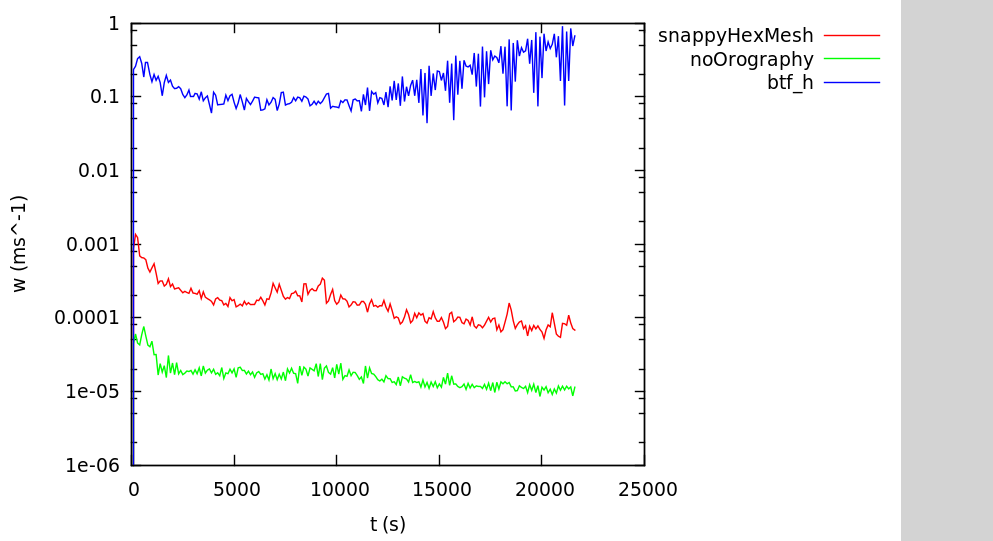
\includegraphics[width=\textwidth]{interim-results/verticalVelocityPlotSnappyHexMesh.png}
\caption{Max vertical velocities (note log scale on y axis)}
\label{fig:rest:w}
\end{figure}

\begin{figure}
BTF H
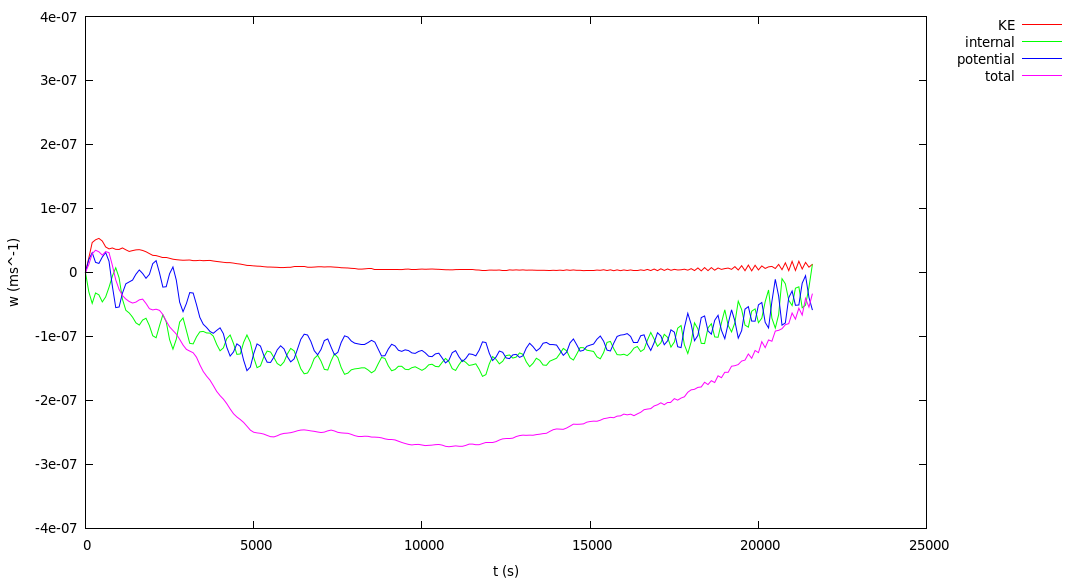
\includegraphics[width=\textwidth]{interim-results/restingBtfHEnergy.png}
SLEVE
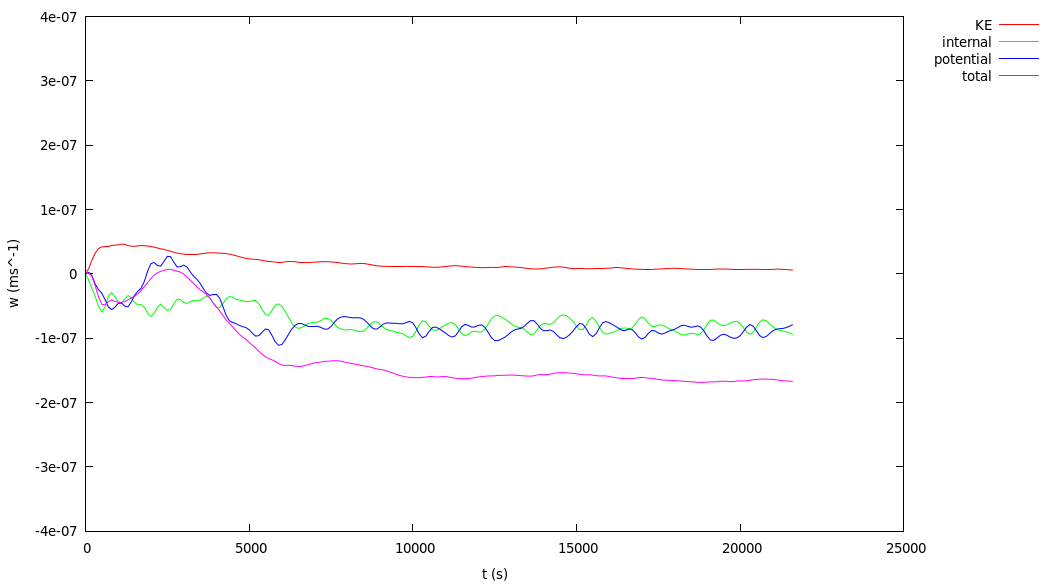
\includegraphics[width=\textwidth]{interim-results/restingSleveEnergy.png}
\caption{Energy changes (TF)}
\label{fig:rest:energy-tf}
\end{figure}

\begin{figure}
SnapCol
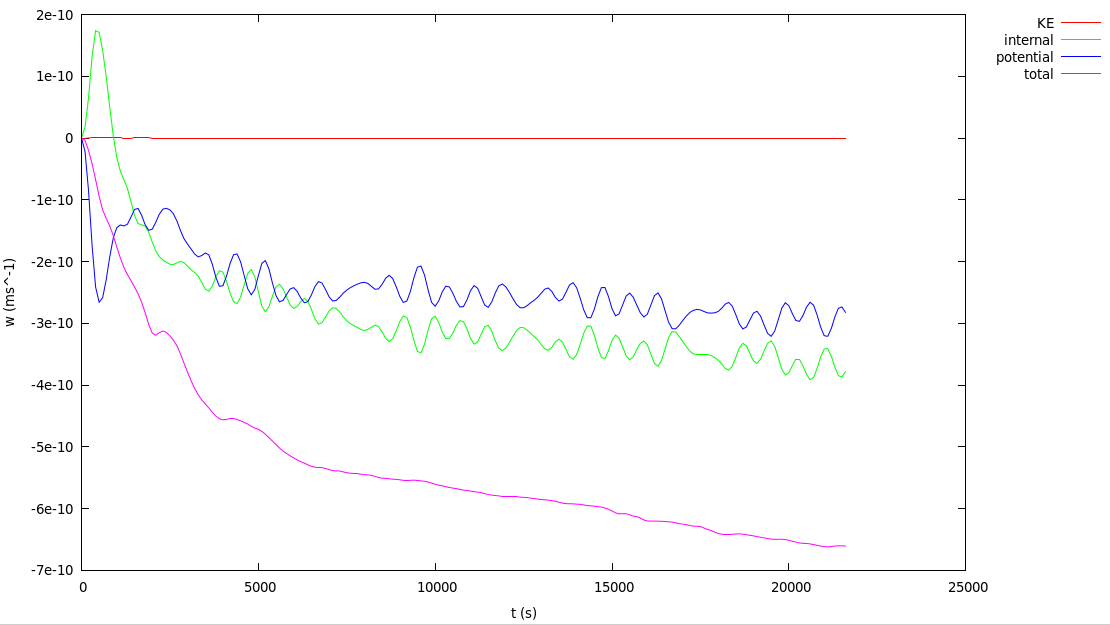
\includegraphics[width=\textwidth]{interim-results/restingSnapColEnergy.png}
Snap
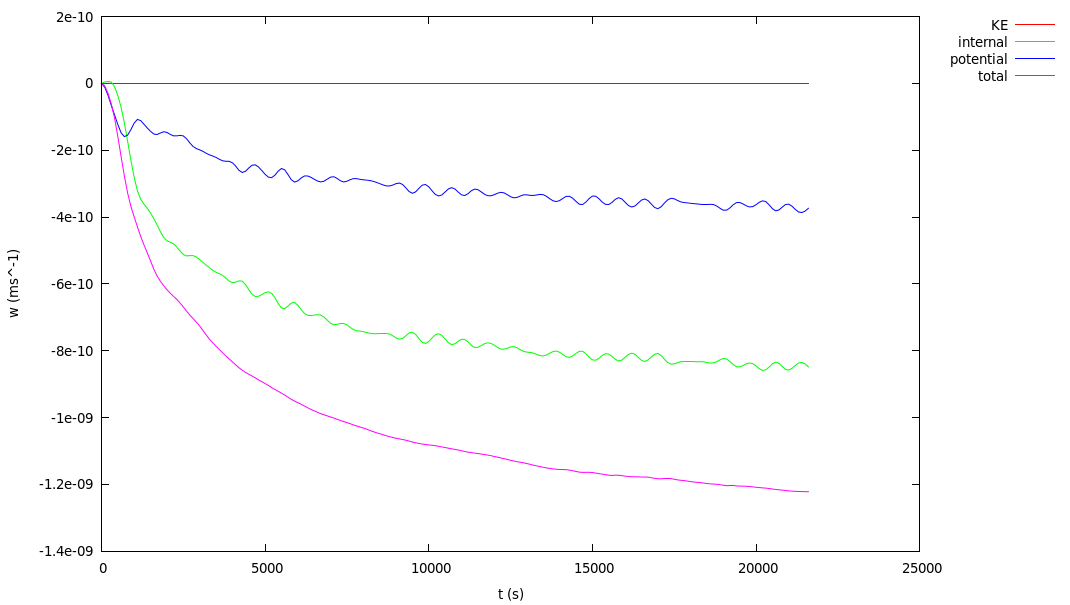
\includegraphics[width=\textwidth]{interim-results/restingSnapEnergy.png}
\caption{Energy changes (cut-cell style)}
\label{fig:rest:energy-cut-cell}
\end{figure}
